\begin{exercice}

 \textsl{Nov. 2005 Am\'erique du Sud} \textbf{Ex.\no 4 Partie A}\\
On consid\`ere les fonctions $f$ et $g$ d\'efinies sur $\R$ par
\[ f(x) = \text{e}^{-x^2} \quad  \text{et}\quad  g(x) = x^2\text{e}^{-x^2}.\]

On note respectivement $\mathcal{C}_{f}$ et $\mathcal{C}_{g}$ les courbes repr\'esentatives de $f$ et $g$ dans un rep\`ere orthogonal $\oij$, dont les trac\'es se trouvent sur la feuille annexe.

\begin{enumerate}
\item  Identifier $\mathcal{C}_{f}$ et $\mathcal{C}_{g}$ sur la figure fournie. (Justifier la r\'eponse apport\'ee).
\item \'Etudier la parit\'e des fonctions $f$ et $g$.
\item \'Etudier le sens de variation de $f$ et de $g$. \'Etudier les limites \'eventuelles de $f$ et de $g$ en $+\infty$.
\item \'Etudier la position relative de $\mathcal{C}_{f}$ et $\mathcal{C}_{g}$.
 \end{enumerate}
%\includegraphics[totalheight=5cm]{courbe_bac_2006}
\includegraphics[totalheight=5cm]{/home/pan/Desktop/TeX_MiX/TS/Chapitres/Exponentielle/Exos/exo-7_3/courbe_bac_2006.eps}
%\includegraphics[totalheight=5cm]{Exoscourbe_bac_2006.jpg}
\end{exercice}
